\section{Overview of Our Approach}\label{sec:overview}

In this paper we present CLgen, a tool for synthesizing OpenCL benchmarks, and an accompanying host driver for executing synthetic benchmarks for gathering performance data for predictive modeling. While we demonstrate our approach using OpenCL, it is language agnostic. Our tool CLgen learns the semantics and structure from over a million lines of hand-written code from GitHub, and synthesizes programs through a process of iterative model sampling. We use a host driver to execute the synthesized programs to gather performance data for use in predictive modeling. Figure~\ref{fig:pipeline} provides an overview of the program synthesis and execution pipeline. Our approach extends the state of the art by providing a general-purpose solution for benchmark synthesis, leading to better and more accurate predictive models.

In the course of evaluating our technique against prior work we discovered that it is also useful for evaluating the quality of features. Since we are able to cover the space so much more finely than the prior work, which only used standard benchmark suites, we are able to find multiple programs with identical feature values but different best heuristic values. This indicates that the features are not sufficiently discriminative and should be extended with more information to allow those programs to be separated. We go on to show that doing this significantly increases the performance of the learned heuristics. We expect that our technique will be valuable for feature designers.

\begin{figure}
  \centering%
  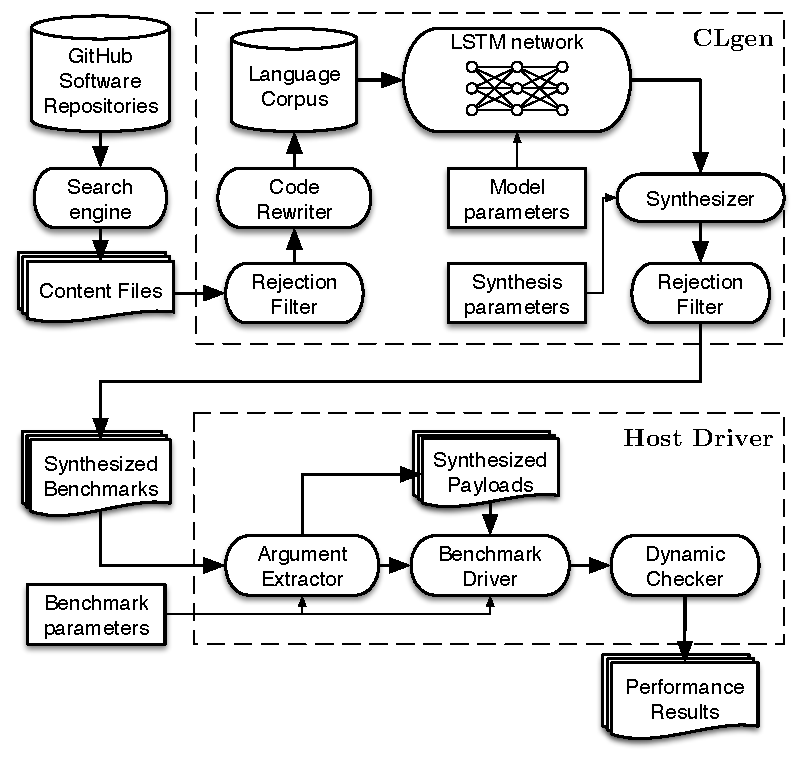
\includegraphics[width=\columnwidth]{img/pipeline}%
  \caption{Benchmark synthesis and execution pipeline.}%
  \label{fig:pipeline}
\end{figure}
